\documentclass[12pt, a4paper, oneside]{ctexart}
\usepackage{amsmath, amsthm, amssymb, bm, color, graphicx, geometry, mathrsfs,extarrows, braket, booktabs, array}
\usepackage[colorlinks,linkcolor=red,anchorcolor=blue,citecolor=blue,urlcolor=blue,menucolor=black]{hyperref}
\setmainfont{Times New Roman}  % 设置英文字体
\setsansfont{Calibri}
\setmonofont{Consolas}

\linespread{1.4}
%\geometry{left=2.54cm,right=2.54cm,top=3.18cm,bottom=3.18cm}
\geometry{left=1.84cm,right=1.84cm,top=2.18cm,bottom=2.18cm}
\newcounter{problem}  % 问题序号计数器
\newenvironment{problem}{\stepcounter{problem}\par\noindent\textbf{题目\arabic{problem}. }}{\smallskip\par}
\newenvironment{solution}{\par\noindent\textbf{解答. }}{\smallskip\par}
\newenvironment{note}{\par\noindent\textbf{注记. }}{\smallskip\par}

%%%% 图片相对路径 %%%%
\graphicspath{{figure/}} % 当前目录下的figure文件夹, {../figure/}则是父目录的figure文件夹

\everymath{\displaystyle} % 默认全部行间公式
\DeclareMathOperator*\uplim{\overline{lim}} % 定义上极限 \uplim_{}
\DeclareMathOperator*\lowlim{\underline{lim}} % 定义下极限 \lowlim_{}
\let\leq=\leqslant % 将全部leq变为leqslant
\let\geq=\geqslant % geq同理

%%%% 一些宏定义 %%%%
\def\bd{\boldsymbol}        % 加粗(向量) boldsymbol
\def\disp{\displaystyle}    % 使用行间公式 displaystyle(默认)
\def\tsty{\textstyle}       % 使用行内公式 textstyle
\def\sign{\text{sign}}      % sign function
\def\wtd{\widetilde}        % 宽波浪线 widetilde
\def\R{\mathbb{R}}          % Real number
\def\N{\mathbb{N}}          % Natural number
\def\Z{\mathbb{Z}}          % Integer number
\def\Q{\mathbb{Q}}          % Rational number
\def\C{\mathbb{C}}          % Complex number
\def\d{\mathrm{d}}          % differential operator
\def\e{\mathrm{e}}          % Euler's number
\def\i{\mathrm{i}}          % imaginary number
\def\re{\mathrm{Re}}        % Real part
\def\im{\mathrm{Im}}        % Imaginary part
\def\res{\mathrm{Res}}      % Residue
\def\L{\mathcal{L}}         % Loss function
\def\wdh{\widehat}          % 宽帽子 widehat
\def\ol{\overline}          % 上横线 overline
\def\ul{\underline}         % 下横线 underline
\def\add{\vspace{1ex}}      % 增加行间距
\def\del{\vspace{-3.5ex}}   % 减少行间距

%%%% 定理类环境的定义 %%%%
\newtheorem{theorem}{定理}

%%%% 基本信息 %%%%
\newcommand{\RQ}{\today} % 日期
\newcommand{\km}{泛函分析} % 科目
\newcommand{\bj}{强基数学002} % 班级
\newcommand{\xm}{吴天阳} % 姓名
\newcommand{\xh}{2204210460} % 学号

\begin{document}

%\pagestyle{empty}
\pagestyle{plain}
\vspace*{-15ex}
\centerline{\begin{tabular}{*5{c}}
    \parbox[t]{0.25\linewidth}{\begin{center}\textbf{日期}\\ \large \textcolor{blue}{\RQ}\end{center}} 
    & \parbox[t]{0.2\linewidth}{\begin{center}\textbf{科目}\\ \large \textcolor{blue}{\km}\end{center}}
    & \parbox[t]{0.2\linewidth}{\begin{center}\textbf{班级}\\ \large \textcolor{blue}{\bj}\end{center}}
    & \parbox[t]{0.1\linewidth}{\begin{center}\textbf{姓名}\\ \large \textcolor{blue}{\xm}\end{center}}
    & \parbox[t]{0.15\linewidth}{\begin{center}\textbf{学号}\\ \large \textcolor{blue}{\xh}\end{center}} \\ \hline
\end{tabular}}
\vspace*{4ex}

% 正文部分
\begin{problem}
    设两个度量空间分别为$(X_1,\rho_1),(X_2,\rho_2)$,映射$T:X_1\to X_2$,证明下述两种函数连续性定义是等价的
    
    1. 任意的数列$\{x_n\}\subset X_1$,若$\exists x\in X_1$,$\rho_1(x_n, x)\to 0$,则有$\rho_2(Tx_n,Tx)\to 0$.

    2. $\forall \varepsilon > 0$,$\forall x_0\in X_1$,$\exists \delta > 0$使得当$\rho_1(x,x_0) < \delta$时$\rho_2(Tx,Tx_0) < \varepsilon$.
\end{problem}
\begin{proof}
    ($1\Rightarrow 2$)反设,$\exists x_0\in X$,$\exists \varepsilon > 0$,使得$\forall n\in \N$,有$\rho_1(x_n,x_0) < \frac{1}{n}$,但$\rho_2(Tx_n,Tx_0)\geq \varepsilon$则$\rho_1(x_n, x_0)\to 0$,由原命题假设可知$\rho_2(Tx_n, Tx_0)\to 0$矛盾.

    ($2\Rightarrow 1$)$\forall \varepsilon > 0$,$\exists N\in \N$,使得$\forall n\geq N$有$\rho_1(x, x_0) < \frac{1}{n}$,有$\rho_2(Tx, Tx_0) < \varepsilon$,令$x_n$满足$\rho_1(x_n,x_0) < \frac{1}{n}$,则由$\varepsilon$的任意性可知$\rho_1(x_n,x_0)\to 0\Rightarrow \rho_2(Tx_n, Tx_0)\to 0$.
\end{proof}
\begin{problem}
    在等距同构的意义下,度量空间的完备化空间是唯一的.
\end{problem}
\begin{proof}
    反设存在$(X_1,\rho_1),(X_2,\rho_2)$为$(X,\rho)$的两个在等距同构下不同的完备化空间,设$T_1:X\to X_1,T_2:X\to X_2$分别为$X$到$X_1$和$X_2$的等距同构映射.
    
    $\forall x_1,x_2\in X_1$,由稠密性可知,存在Cauchy列$\{x_{n1}\},\{x_{n2}\}\subset X$使得$T_1x_{n1}\to x_1,T_2x_{n2}\to x_2$,由等距性可知
    \begin{align*}
        \rho(x_{n1}, x_{n2}) = \rho_1(T_1x_{n1}, T_2x_{n2}) = \rho_1(T_1x_{n1},x_1)+\rho_1(x_1,x_2)+\rho_1(x_2,Tx_{n2}) = \rho_1(x_1,x_2),\quad(n\to \infty)
    \end{align*}
    由于$\{x_{n1}\},\{x_{n2}\}$均为Cauchy列,则存在$x_1',x_2'\in X_2$,使得$T_2x_{n1}\to x_1',T_2x_{n2}\to x_2'$,类似地有
    \begin{equation*}
        \rho(x_{n1},x_{n2}) = \rho_2(x_1',x_2'),\quad(n\to \infty)
    \end{equation*}
    于是$\rho_1(x_1,x_2) = \rho_2(x_1',x_2')$.

    由$x_1,x_2$的任意性,可构造等距同构映射$T' = T_2(T_1^{-1}):X_1\to X_2$,则$T'^{-1} = T_1(T_2^{-1})$,且$\forall x_1,x_2\in X_1$有$\rho_1(x_1,x_2) = \rho_2(T'x_1,T'x_2)$. 故度量空间$X_1$与$X_2$在$T'$下等距同构,与假设矛盾. 所以度量空间的完备化空间是唯一的.
\end{proof}
\begin{problem}
    设 $C_0^1(0, 1):=\{f\in C^1(0, 1): f\text{在}0\text{和}1\text{的某领域上等于}0\}$,定义
    \begin{equation*}
        \rho(x, y) = \left(\int_0^1(|x(t)-y(t)|^2+|x'(t)-y'(t)|^2)\,\d x\right)^{1/2}
    \end{equation*}

    1. $(C_0^1(0, 1), \rho)$是一个度量空间,但不完备.
    
    2. 设$X$是$C_0^1(0,1)$在$\rho$下的完备化空间,证明$X\subset C[0,1]$.
\end{problem}
\begin{proof}
    1. (正定性)$\forall x, y, z\in C_0^1(0, 1)$在$(0,1)$上有$|x-y|^2+|x'-y'|^2\geq 0$,于是$\rho(x, y)\geq 0$. 又由于$\rho(x, y) = 0\iff x=y, x'=y', a.e.\iff x=y\ \text{(连续性)}$.
    
    (对称性)由于$|x-y| = |y-x|$,于是$\rho(x, y) = \rho(y, x)$.

    (三角不等式)要证$\rho(x, y)\leq \rho(x, z)+\rho(z, y)$,只需证$\rho(x,y)^2\leq \rho(x, z)^2+2\rho(x,z)\rho(z,y)+\rho(z,y)^2$,由于
    \begin{align*}
        &\ \rho(x,z)^2+2\rho(x,z)\rho(z,y)+\rho(z,y)^2\\
        = &\ \int_0^1(|x-z|^2+|x'-z'|^2)\,\d t+2\left(\int_0^1(|x-z|^2+|x'-z'|^2)\,\d t\int_0^1(|z-y|^2+|z'-y'|^2)\,\d t\right)^{1/2}\\
        &\hspace{5cm}+\int_0^1(|z-y|^2+|z'-y'|^2)\,\d t
    \end{align*}
    使用两次Cauchy-Schwarz不等式可知
    \begin{align*}
        &\ \left(\int_0^1(|x-z|^2+|x'-z'|^2)\,\d t\int_0^1(|z-y|^2+|z'-y'|^2)\,\d t\right)^{1/2}\\
        \text{(积分形式不等式)}\geq&\ \int_0^1\sqrt{|x-z|^2+|x'-z'|^2}\sqrt{|z-y|^2+|z'-y'|^2}\,\d t\\
        \text{(求和形式不等式)}\geq&\ \int_0^1|x-z||z-y|+|x'-z'||z'-y'|\,\d t
    \end{align*}
    于是
    \begin{align*}
        &\ \rho(x, z)^2+2\rho(x,z)\rho(z,y)+\rho(z,y)^2\\
        \geq&\ \int_0^1(|x-z|^2+2|x-z||z-y|+|z-y|^2)\,\d t+\int_0^1(|x'-z'|^2+2|x'-z'||z'-y'|+|z'-y'|^2)\,\d t\\
        \geq&\ \int_0^1(|x-z|+|z-y|)^2\,\d t+\int_0^1(|x'-z'|+|z'-y'|)^2\,\d t\\
        \geq&\ \int_0^1(|x-y|^2+|x'-y'|^2)\,\d  t = \rho(x, y)^2
    \end{align*}
\end{proof}
\begin{problem}
    证明$L^{\infty}[a,b]$不可分.
\end{problem}
\begin{note}
    $L^{\infty}[a,b]:=\{f\text{可测}:\inf_{m(E_0)=0}\sup_{x\in[a,b]-E_0}|f(x)| < \infty\}$).
\end{note}
\begin{proof}
    $L^{\infty}[a,b]$中测度为$\rho(f,g):=\inf_{m(E_0)=0}\sup_{x\in[a,b]-E_0}|f(x)-g(x)|$.
    
    不妨令$a=0, b=1$,类似证明$l^{\infty}$的思路. 构造不可数集合
    \begin{equation*}
        S = \left\{\lim_{n\to\infty}\sum_{i=1}^n\xi_i\cdot \chi_{\left[0,\frac{i}{n}\right]}:\xi_i\in\{0,1\}\right\}
    \end{equation*}
    其中$\chi_{[a,b]}$表示在$[a,b]$上取值为$1$其他位置为$0$的函数. 由于$S$与二进制序列等势,则$\ol{\ol{S}}=\aleph$,且$\rho(f, g) = 1,\ f, g\in S, f\neq g$.

    假设$L^{\infty}$不可分,则存在$\{h_n\}\subset L^{\infty}$,使得$\{h_n\}$在$L^\infty$中稠密,于是$S\subset \bigcup_{n\geq 1}B(h_n,1/3)$,由于$S$不可数,则必存在正整数$i$和$S$中的两个不同函数$f,g$,使得$f,g\in B(h_i, 1/3)$,则$\rho(f,g)\leq 2/3$与$\rho(f,g)=1$矛盾,故$L^\infty$不可分.
\end{proof}

\begin{problem}
    证明$l^p(1\leq p < \infty)$可分.
\end{problem}
\begin{note}
$l^p:=\{\text{数列}\{x_n\}:\sum_{i=1}^\infty |x_i|^p < \infty\}$,其上的度量为$\rho(\xi,\mu) = \left(\sum_{i=1}^n|x_i-y_i|^p\right)^{1/p},\ (\xi = \{x_n\}, \mu = \{y_n\})$
\end{note}
\begin{proof}
    设$S = \{(q_1,q_2,\cdots,q_n,0,0,\cdots):q_i\in\Q, n\in\N\}$,则$S$为可数集,下证$S$在$l^p$中稠密.\add

    $\forall \xi \in l^p$,令$\xi=(x_1,x_2,\cdots)$,由于$\sum_{i=1}^\infty |x_i|^p < \infty$,则$\forall \varepsilon > 0$,$\exists N\in\N$使得$\sum_{i=N+1}^\infty|x_i|^p < \varepsilon^p$,由于$\Q$在$\R$中稠密,可以取到
    \begin{equation*}
        \eta = (q_1,q_2,\cdots, q_N,0,0,\cdots)\in S 
    \end{equation*}
    且满足$|q_i-x_i|^p < \frac{\varepsilon^p}{2^i}$,于是
    \begin{align*}
        \rho(\xi,\eta)=&\ \left(\sum_{i=1}^N|x_i-q_i|^p+\sum_{i=N+1}^\infty|x_i|^p\right)^{1/p}\\
        \leq&\ \left(\sum_{i=1}^\infty\frac{\varepsilon^p}{2^i}+\varepsilon^p\right)^{1/p}\\
        =&\ (2\varepsilon^p)^{1/p} = 2^{1/p}\varepsilon\to 0.
    \end{align*}
    说明可数集$S$是$l^p$上的稠密子集,则$l^p$是可分的.
\end{proof}

% 下面给一些功能的写法
\iffalse
% 图片模板
\centerline{
    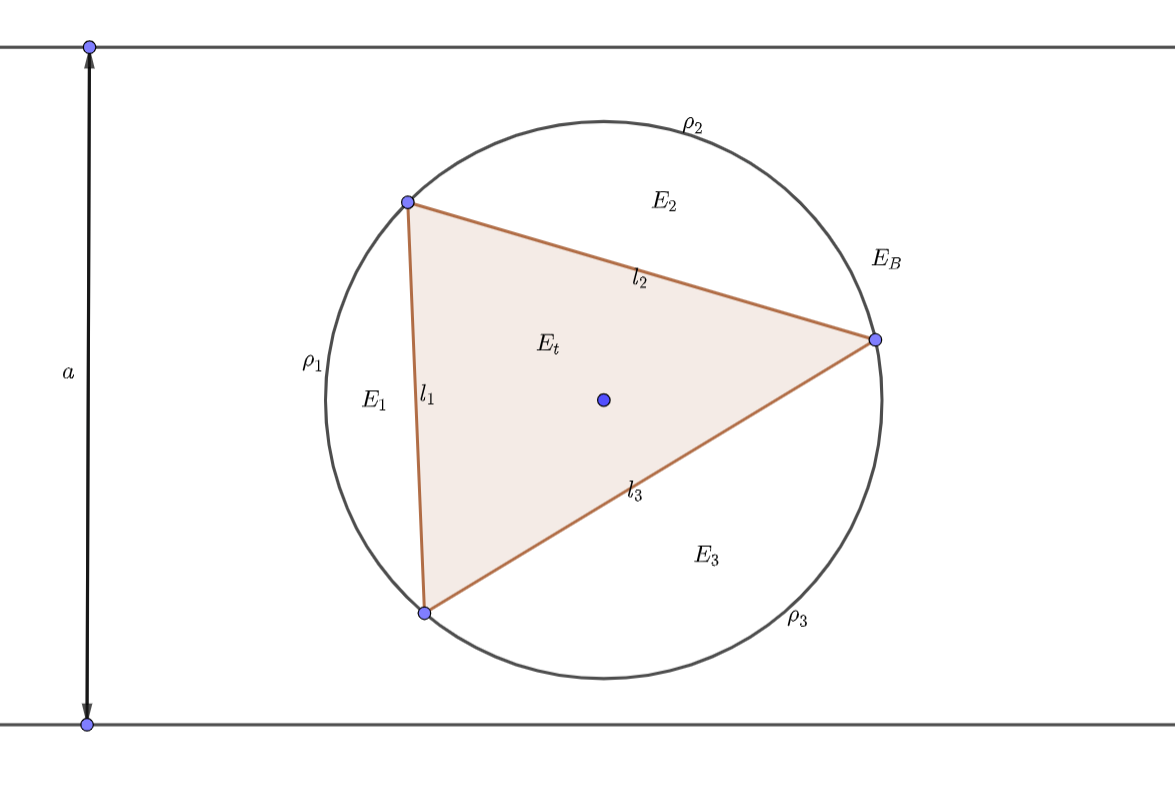
\includegraphics[width=0.8\textwidth]{figure.png}
}
% 表格模板
\renewcommand\arraystretch{0.8} % 设置表格高度为原来的0.8倍
\begin{table}[!htbp] % table标准
    \centering % 表格居中
    \begin{tabular}{p{1cm}<{\centering}p{1cm}<{\centering}p{3cm}<{\centering}p{5cm}<{\centering}} % 设置表格宽度
    %\begin{tabular}{cccc}
        \toprule
        $x_i$ & $f[x_1]$ & $f[x_i,x_{i+1}]$ & $f[x_i,x_{i+1},x_{i+2}]$ \\
        \midrule
        $x_0$ & $f(x_0)$ &                  &                          \\
        $x_0$ & $f(x_0)$ & $f'(x_0)$        &                          \\
        $x_0$ & $f(x_1)$ & $\frac{f(x_1)-f(x_0)}{x_1-x_0}$ & $\frac{f(x_1)-f(x_0)}{(x_1-x_0)^2}-\frac{f'(x_0)}{x_1-x_0}$\\
        \bottomrule
    \end{tabular}
\end{table}

\def\Log{\text{Log}} % 一个简单的宏定义
$\Log$ % 调用方法
\fi

\end{document}